        %%******************************************%%
        %%                                          %%
        %%        Modello di tesi di laurea         %%
        %%            di Andrea Giraldin            %%
        %%                                          %%
        %%             2 novembre 2012              %%
        %%                                          %%
        %%******************************************%%


% I seguenti commenti speciali impostano:
% 1. 
% 2. PDFLaTeX come motore di composizione;
% 3. tesi.tex come documento principale;
% 4. il controllo ortografico italiano per l'editor.

% !TEX encoding = UTF-8
% !TEX TS-program = pdflatex
% !TEX root = tesi.tex
% !TEX spellcheck = it-IT

% PDF/A filecontents
\RequirePackage{filecontents}
\begin{filecontents*}{\jobname.xmpdata}
  \Title{Integrazione di Single Sign-On in Linux Pluggable Authentication Module (Linux PAM)}
  \Author{Ivan Antonino Arena}
  \Language{it-IT}
  \Subject{Lo scopo della tesi è illustrare il lavoro eseguito con Athesys,
    system integrator specializzato nello sviluppo di soluzioni di Identity and Access Management (IAM),
    in termini di innovazione e ricerca applicate all'ambito dell'integrazione di servizi web con sistemi unix-based.
    Nello specifico, si discute la collaborazione con il team infrastructure ed il team dedicato 
    alla ricerca in materia di identità digitale e la conseguente realizzazione di un componente
    Single Sign-On compatibile con Linux Pluggable Authentication Module (Linux PAM).}
  \Keywords{Single Sign-On\sep SSI\sep PAM\sep Unix\sep C}
\end{filecontents*}

\documentclass[10pt,                    % corpo del font principale
               a4paper,                 % carta A4
               twoside,                 % impagina per fronte-retro
               openright,               % inizio capitoli a destra
               english,                 
               italian,                 
               ]{book}    

%**************************************************************
% Importazione package
%************************************************************** 

\PassOptionsToPackage{dvipsnames}{xcolor} % colori PDF/A

\usepackage{colorprofiles}

\usepackage[a-2b,mathxmp]{pdfx}[2018/12/22]
                                        % configurazione PDF/A
                                        % validare in https://www.pdf-online.com/osa/validate.aspx

%\usepackage{amsmath,amssymb,amsthm}    % matematica

\usepackage[T1]{fontenc}                % codifica dei font:
                                        % NOTA BENE! richiede una distribuzione *completa* di LaTeX

\usepackage[utf8]{inputenc}             % codifica di input; anche [latin1] va bene
                                        % NOTA BENE! va accordata con le preferenze dell'editor

\usepackage[english, italian]{babel}    % per scrivere in italiano e in inglese;
                                        % l'ultima lingua (l'italiano) risulta predefinita

\usepackage{bookmark}                   % segnalibri

\usepackage{caption}                    % didascalie

\usepackage{chngpage,calc}              % centra il frontespizio

\usepackage{csquotes}                   % gestisce automaticamente i caratteri (")

\usepackage{emptypage}                  % pagine vuote senza testatina e piede di pagina

\usepackage{epigraph}			% per epigrafi

\usepackage{eurosym}                    % simbolo dell'euro

%\usepackage{indentfirst}               % rientra il primo paragrafo di ogni sezione

\usepackage{graphicx}                   % immagini

\usepackage{hyperref}                   % collegamenti ipertestuali

\usepackage[binding=5mm]{layaureo}      % margini ottimizzati per l'A4; rilegatura di 5 mm

\usepackage{listings}                   % codici

\usepackage{microtype}                  % microtipografia

\usepackage{mparhack,fixltx2e,relsize}  % finezze tipografiche

\usepackage{nameref}                    % visualizza nome dei riferimenti                                      
\usepackage[font=small]{quoting}        % citazioni

\usepackage{subfig}                     % sottofigure, sottotabelle

\usepackage[italian]{varioref}          % riferimenti completi della pagina

\usepackage{booktabs}                   % tabelle                                       
\usepackage{tabularx}                   % tabelle di larghezza prefissata                                    
\usepackage{longtable}                  % tabelle su più pagine                                        
\usepackage{ltxtable}                   % tabelle su più pagine e adattabili in larghezza

\usepackage[toc, acronym]{glossaries}   % glossario
                                        % per includerlo nel documento bisogna:
                                        % 1. compilare una prima volta tesi.tex;
                                        % 2. eseguire: makeindex -s tesi.ist -t tesi.glg -o tesi.gls tesi.glo
                                        % 3. eseguire: makeindex -s tesi.ist -t tesi.alg -o tesi.acr tesi.acn
                                        % 4. compilare due volte tesi.tex.

\usepackage[backend=biber,style=numeric-comp,hyperref,backref]{biblatex}
                                        % eccellente pacchetto per la bibliografia; 
                                        % produce uno stile di citazione autore-anno; 
                                        % lo stile "numeric-comp" produce riferimenti numerici
                                        % per includerlo nel documento bisogna:
                                        % 1. compilare una prima volta tesi.tex;
                                        % 2. eseguire: biber tesi
                                        % 3. compilare ancora tesi.tex.

%**************************************************************
% file contenente le impostazioni della tesi
%**************************************************************

%**************************************************************
% Frontespizio
%**************************************************************

% Autore
\newcommand{\myName}{Ivan Antonino Arena}                                    
\newcommand{\myTitle}{Integrazione di Single Sign-On in Unix Pluggable Authentication Module (Linux PAM)}

% Tipo di tesi                   
\newcommand{\myDegree}{Tesi di laurea}

% Università             
\newcommand{\myUni}{Università degli Studi di Padova}

% Facoltà       
\newcommand{\myFaculty}{Corso di Laurea in Informatica}

% Dipartimento
\newcommand{\myDepartment}{Dipartimento di Matematica "Tullio Levi-Civita"}

% Titolo del relatore
\newcommand{\profTitle}{Prof. }

% Relatore
\newcommand{\myProf}{Davide Bresolin}

% Luogo
\newcommand{\myLocation}{Padova}

% Anno accademico
\newcommand{\myAA}{2022-2023}

% Data discussione
\newcommand{\myTime}{Maggio 2023}

\newcommand{\myAzienda}{Athesys Srl}


%**************************************************************
% Impostazioni di impaginazione
% see: http://wwwcdf.pd.infn.it/AppuntiLinux/a2547.htm
%**************************************************************

\setlength{\parindent}{14pt}   % larghezza rientro della prima riga
\setlength{\parskip}{0pt}   % distanza tra i paragrafi


%**************************************************************
% Impostazioni di biblatex
%**************************************************************
\bibliography{bibliografia} % database di biblatex 

\defbibheading{bibliography} {
    \cleardoublepage
    \phantomsection 
    \addcontentsline{toc}{chapter}{\bibname}
    \chapter*{\bibname\markboth{\bibname}{\bibname}}
}

\setlength\bibitemsep{1.5\itemsep} % spazio tra entry

\DeclareBibliographyCategory{opere}
\DeclareBibliographyCategory{web}

\addtocategory{opere}{womak:lean-thinking}
\addtocategory{web}{site:agile-manifesto}

\defbibheading{opere}{\section*{Riferimenti bibliografici}}
\defbibheading{web}{\section*{Siti Web consultati}}


%**************************************************************
% Impostazioni di caption
%**************************************************************
\captionsetup{
    tableposition=top,
    figureposition=bottom,
    font=small,
    format=hang,
    labelfont=bf
}

%**************************************************************
% Impostazioni di glossaries
%**************************************************************
\makeglossaries

%**************************************************************
% Acronimi
%**************************************************************
\newacronym[description={\glslink{cli}{Command-Line Interface}}]
    {cli}{CLI}{Command-Line Interface}

\newacronym[description={\glslink{sso}{Single Sign-On}}]
    {sso}{SSO}{Single Sign-On}

\newacronym[description={\glslink{ssi}{Self-Sovereign Identity}}]
    {ssi}{SSI}{Self-Sovereign Identity}

\newacronym[description={\glslink{rhel}{Red Hat Enterprise Linux
}}]
    {rhel}{RHEL}{Red Hat Enterprise Linux}

\newacronym[description={\glslink{centos}{Community Enterprise Operating System
}}]
    {centos}{CentOS}{Community Enterprise Operating System}

\newacronym[description={\glslink{saas}{Software as a Service
}}]
    {saas}{SaaS}{Software as a Service}

\newacronym[description={\glslink{iam}{Identity and Access Management}}]
    {iam}{IAM}{Identity and Access Management}

\newacronym[description={\glslink{ldap}{Lightweight Directory Access Protocol}}]
    {ldap}{LDAP}{Lightweight Directory Access Protocol}

\newacronym[description={\glslink{mit}{Massachusetts Institute of Technology}}]
    {mit}{MIT}{Massachusetts Institute of Technology}

\newacronym[description={\glslink{ntp}{Network Time Protocol}}]
    {ntp}{NTP}{Network Time Protocol}

\newacronym[description={\glslink{dns}{Domain Name System}}]
    {dns}{DNS}{Domain Name System}

\newacronym[description={\glslink{sssd}{System Security Services Daemon}}]
    {sssd}{SSSD}{System Security Services Daemon}

\newacronym[description={\glslink{pam}{Pluggable Authentication Modules}}]
    {pam}{PAM}{Pluggable Authentication Modules}

\newacronym[description={\glslink{oauth2}{Open Authorization 2.0}}]
    {oauth2}{OAuth2}{Open Authorization 2.0}

\newacronym[description={\glslink{oidc}{OpenID Connect}}]
    {oidc}{OIDC}{OpenID Connect}

\newacronym[description={\glslink{ssh}{Secure Shell}}]
    {ssh}{SSH}{Secure Shell}

\newacronym[description={\glslink{lxc}{Linux Containers}}]
    {lxc}{LXC}{Linux Containers}

\newacronym[description={\glslink{pve}{Proxmox Virtual Environment}}]
    {pve}{PVE}{Proxmox Virtual Environment}

\newacronym[description={\glslink{kvm}{Kernel-based Virtual Machine}}]
    {kvm}{KVM}{Kernel-based Virtual Machine}

\newacronym[description={\glslink{idaas}{Identity as a Service}}]{idaas}{IDaaS}{Identity as a Service}

\newacronym[description={\glslink{saml}{Security Assertion Markup Language}}]{saml}{SAML}{Security Assertion Markup Language}

\newacronym[description={\glslink{did}{Decentralized Identifier}}]{did}{DID}{Decentralized Identifier}

\newacronym[description={\glslink{cto}{Chief Technology Officer}}]{cto}{CTO}{Chief Technology Officer}

\newacronym[description={\glslink{poc}{Proof of Concept}}]{poc}{PoC}{Proof of Concept}

\newacronym[description={\glslink{idp}{Identity Provider}}]{idp}{IdP}{Identity Provider}

\newacronym[description={\glslink{gui}{Graphical User Interface}}]{gui}{GUI}{Graphical User Interface}

\newacronym[description={\glslink{lts}{Long-term Support}}]{lts}{LTS}{Long-term Support}



%**************************************************************
% Glossario
%**************************************************************

% \newglossaryentry{umlg}
% {
%     name=\glslink{uml}{UML},
%     text=UML,
%     sort=uml,
%     description={in ingegneria del software \emph{UML, Unified Modeling Language} (ing. linguaggio di modellazione unificato) è un linguaggio di modellazione e specifica basato sul paradigma object-oriented. L'\emph{UML} svolge un'importantissima funzione di ``lingua franca'' nella comunità della progettazione e programmazione a oggetti. Gran parte della letteratura di settore usa tale linguaggio per descrivere soluzioni analitiche e progettuali in modo sintetico e comprensibile a un vasto pubblico}
% }
 % database di termini


%**************************************************************
% Impostazioni di graphicx
%**************************************************************
\graphicspath{{immagini/}} % cartella dove sono riposte le immagini


%**************************************************************
% Impostazioni di hyperref
%**************************************************************
\hypersetup{
    %hyperfootnotes=false,
    %pdfpagelabels,
    %draft,	% = elimina tutti i link (utile per stampe in bianco e nero)
    colorlinks=true,
    linktocpage=true,
    pdfstartpage=1,
    pdfstartview=,
    % decommenta la riga seguente per avere link in nero (per esempio per la stampa in bianco e nero)
    %colorlinks=false, linktocpage=false, pdfborder={0 0 0}, pdfstartpage=1, pdfstartview=FitV,
    breaklinks=true,
    pdfpagemode=UseNone,
    pageanchor=true,
    pdfpagemode=UseOutlines,
    plainpages=false,
    bookmarksnumbered,
    bookmarksopen=true,
    bookmarksopenlevel=1,
    hypertexnames=true,
    pdfhighlight=/O,
    %nesting=true,
    %frenchlinks,
    urlcolor=webbrown,
    linkcolor=RoyalBlue,
    citecolor=webgreen,
    %pagecolor=RoyalBlue,
    %urlcolor=Black, linkcolor=Black, citecolor=Black, %pagecolor=Black,
    pdftitle={\myTitle},
    pdfauthor={\textcopyright\ \myName, \myUni, \myFaculty},
    pdfsubject={},
    pdfkeywords={},
    pdfcreator={pdfLaTeX},
    pdfproducer={LaTeX}
}

%**************************************************************
% Impostazioni di itemize
%**************************************************************
\renewcommand{\labelitemi}{$\ast$}

%\renewcommand{\labelitemi}{$\bullet$}
%\renewcommand{\labelitemii}{$\cdot$}
%\renewcommand{\labelitemiii}{$\diamond$}
%\renewcommand{\labelitemiv}{$\ast$}


%**************************************************************
% Impostazioni di listings
%**************************************************************
\lstset{
    language=[LaTeX]Tex,C,
    keywordstyle=\color{RoyalBlue}, %\bfseries,
    basicstyle=\small\ttfamily,
    %identifierstyle=\color{NavyBlue},
    commentstyle=\color{Green}\ttfamily,
    stringstyle=\rmfamily,
    numbers=none, %left,%
    numberstyle=\scriptsize, %\tiny
    stepnumber=5,
    numbersep=8pt,
    showstringspaces=false,
    breaklines=true,
    frameround=ftff,
    frame=single
} 


%**************************************************************
% Impostazioni di xcolor
%**************************************************************
\definecolor{webgreen}{rgb}{0,.5,0}
\definecolor{webbrown}{rgb}{.6,0,0}


%**************************************************************
% Altro
%**************************************************************

\newcommand{\omissis}{[\dots\negthinspace]} % produce [...]

% eccezioni all'algoritmo di sillabazione
\hyphenation
{
    ma-cro-istru-zio-ne
    gi-ral-din
}

\newcommand{\sectionname}{sezione}
\addto\captionsitalian{\renewcommand{\figurename}{Figura}
                       \renewcommand{\tablename}{Tabella}}

\newcommand{\glsfirstoccur}{\ap{{[g]}}}

\newcommand{\intro}[1]{\emph{\textsf{#1}}}

%**************************************************************
% Environment per ``rischi''
%**************************************************************
\newcounter{riskcounter}                % define a counter
\setcounter{riskcounter}{0}             % set the counter to some initial value

%%%% Parameters
% #1: Title
\newenvironment{risk}[1]{
    \refstepcounter{riskcounter}        % increment counter
    \par \noindent                      % start new paragraph
    \textbf{\arabic{riskcounter}. #1}   % display the title before the 
                                        % content of the environment is displayed 
}{
    \par\medskip
}

\newcommand{\riskname}{Rischio}

\newcommand{\riskdescription}[1]{\textbf{\\Descrizione:} #1.}

\newcommand{\risksolution}[1]{\textbf{\\Soluzione:} #1.}

%**************************************************************
% Environment per ``use case''
%**************************************************************
\newcounter{usecasecounter}             % define a counter
\setcounter{usecasecounter}{0}          % set the counter to some initial value

%%%% Parameters
% #1: ID
% #2: Nome
\newenvironment{usecase}[2]{
    \renewcommand{\theusecasecounter}{\usecasename #1}  % this is where the display of 
                                                        % the counter is overwritten/modified
    \refstepcounter{usecasecounter}             % increment counter
    \vspace{10pt}
    \par \noindent                              % start new paragraph
    {\large \textbf{\usecasename #1: #2}}       % display the title before the 
                                                % content of the environment is displayed 
    \medskip
}{
    \medskip
}

\newcommand{\usecasename}{UC}

\newcommand{\usecaseactors}[1]{\textbf{\\Attori Principali:} #1. \vspace{4pt}}
\newcommand{\usecasepre}[1]{\textbf{\\Precondizioni:} #1. \vspace{4pt}}
\newcommand{\usecasedesc}[1]{\textbf{\\Descrizione:} #1. \vspace{4pt}}
\newcommand{\usecasepost}[1]{\textbf{\\Postcondizioni:} #1. \vspace{4pt}}
\newcommand{\usecasealt}[1]{\textbf{\\Scenario Alternativo:} #1. \vspace{4pt}}

%**************************************************************
% Environment per ``namespace description''
%**************************************************************

\newenvironment{namespacedesc}{
    \vspace{10pt}
    \par \noindent                              % start new paragraph
    \begin{description} 
}{
    \end{description}
    \medskip
}

\newcommand{\classdesc}[2]{\item[\textbf{#1:}] #2}
                     % file con le impostazioni personali

\begin{document}
%**************************************************************
% Materiale iniziale
%**************************************************************
\frontmatter
% !TEX encoding = UTF-8
% !TEX TS-program = pdflatex
% !TEX root = ../tesi.tex

%**************************************************************
% Frontespizio 
%**************************************************************
\begin{titlepage}

\begin{center}

\begin{LARGE}
\textbf{\myUni}\\
\end{LARGE}

\vspace{10pt}

\begin{Large}
\textsc{\myDepartment}\\
\end{Large}

\vspace{10pt}

\begin{large}
\textsc{\myFaculty}\\
\end{large}

\vspace{30pt}
\begin{figure}[htbp]
\begin{center}

\includegraphics[height=6cm]{logo-unipd}
\end{center}
\end{figure}
\vspace{30pt} 

\begin{LARGE}
\begin{center}
\textbf{\myTitle}\\
\end{center}
\end{LARGE}

\vspace{10pt} 

\begin{large}
\textsl{\myDegree}\\
\end{large}

\vspace{40pt} 

\begin{large}
\begin{flushleft}
\textit{Relatore}\\ 
\vspace{5pt} 
\profTitle \myProf
\end{flushleft}

\vspace{0pt} 

\begin{flushright}
\textit{Laureando}\\ 
\vspace{5pt} 
\myName
\end{flushright}
\end{large}

\vspace{40pt}

\line(1, 0){338} \\
\begin{normalsize}
\textsc{Anno Accademico \myAA}
\end{normalsize}

\end{center}
\end{titlepage} 
% !TEX encoding = UTF-8
% !TEX TS-program = pdflatex
% !TEX root = ../tesi.tex

%**************************************************************
% Colophon
%**************************************************************
\clearpage
\phantomsection
\thispagestyle{empty}

\hfill

\vfill

\noindent\myName: \textit{\myTitle,}
\myDegree,
\textcopyright\ \myTime.
% !TEX encoding = UTF-8
% !TEX TS-program = pdflatex
% !TEX root = ../tesi.tex

%**************************************************************
% Dedica
%**************************************************************
\cleardoublepage
\phantomsection
\thispagestyle{empty}
\pdfbookmark{Dedica}{Dedica}

\vspace*{3cm}

\begin{center}
Lorem ipsum dolor sit amet, consectetuer adipiscing elit. \\ \medskip
--- Oscar Wilde    
\end{center}

\medskip

\begin{center}
Dedicato a ...
\end{center}

\let\cleardoublepage\clearpage
% !TEX encoding = UTF-8
% !TEX TS-program = pdflatex
% !TEX root = ../tesi.tex

%**************************************************************
% Sommario
%**************************************************************
\cleardoublepage
\phantomsection
\pdfbookmark{Abstract}{Abstract}
\begingroup
\let\clearpage\relax
\let\cleardoublepage\relax
\let\cleardoublepage\relax

\chapter*{Abstract}

Lo scopo della tesi è illustrare il lavoro eseguito con Athesys, system integrator specializzato nello sviluppo di soluzioni di Identity and Access Management (IAM), in termini di innovazione e ricerca applicate all'ambito dell'integrazione di servizi web con sistemi unix-based. Nello specifico, si discute la collaborazione con il team infrastructure ed il team dedicato alla ricerca in materia di identità digitale e la conseguente realizzazione di un componente Single Sign-On compatibile con Linux Pluggable Authentication Module (Linux PAM). ​

%\vfill
%
%\selectlanguage{english}
%\pdfbookmark{Abstract}{Abstract}
%\chapter*{Abstract}
%
%\selectlanguage{italian}

\endgroup			

\vfill


% !TEX encoding = UTF-8
% !TEX TS-program = pdflatex
% !TEX root = ../tesi.tex

%**************************************************************
% Ringraziamenti
%**************************************************************
\cleardoublepage
\phantomsection
\pdfbookmark{Ringraziamenti}{ringraziamenti}

\begin{flushright}{
	\slshape    
	``Life is really simple, but we insist on making it complicated''} \\ 
	\medskip
    --- Confucius
\end{flushright}


\bigskip

\begingroup
\let\clearpage\relax
\let\cleardoublepage\relax
\let\cleardoublepage\relax

\chapter*{Ringraziamenti}

\noindent \textit{Innanzitutto, vorrei esprimere la mia gratitudine al Prof. NomeDelProfessore, relatore della mia tesi, per l'aiuto e il sostegno fornitomi durante la stesura del lavoro.}\\

\noindent \textit{Desidero ringraziare con affetto i miei genitori per il sostegno, il grande aiuto e per essermi stati vicini in ogni momento durante gli anni di studio.}\\

\noindent \textit{Ho desiderio di ringraziare poi i miei amici per tutti i bellissimi anni passati insieme e le mille avventure vissute.}\\
\bigskip

\noindent\textit{\myLocation, \myTime}
\hfill \myName

\endgroup


% !TEX encoding = UTF-8
% !TEX TS-program = pdflatex
% !TEX root = ../tesi.tex

%**************************************************************
% Indici
%**************************************************************
\cleardoublepage
\pdfbookmark{\contentsname}{tableofcontents}
\setcounter{tocdepth}{2}
\tableofcontents
%\markboth{\contentsname}{\contentsname} 
\clearpage

\begingroup 
    \let\clearpage\relax
    \let\cleardoublepage\relax
    \let\cleardoublepage\relax
    %*******************************************************
    % Elenco delle figure
    %*******************************************************    
    \phantomsection
    \pdfbookmark{\listfigurename}{lof}
    \listoffigures

    \vspace*{8ex}

    %*******************************************************
    % Elenco delle tabelle
    %*******************************************************
    % \phantomsection
    % \pdfbookmark{\listtablename}{lot}
    % \listoftables
        
    % \vspace*{8ex}
\endgroup

\cleardoublepage


%**************************************************************
% Materiale principale
%**************************************************************
\mainmatter
% !TEX encoding = UTF-8
% !TEX TS-program = pdflatex
% !TEX root = ../tesi.tex

%**************************************************************
\chapter{Introduzione}
\label{cap:introduzione}
%**************************************************************

\intro{In questo capitolo vengono descritti l'azienda ospitante ed il progetto dell'attività di stage curriculare.}


% \noindent Esempio di utilizzo di un termine nel glossario \\
% \gls{api}. \\

% \noindent Esempio di citazione in linea \\
% \cite{site:agile-manifesto}. \\

% \noindent Esempio di citazione in linea \\
% \cite{site:what-is-oauth}. \\

% \noindent Esempio di citazione nel pie' di pagina \\
% citazione\cite{womak:lean-thinking} \\

%**************************************************************
\section{L'azienda}

Athesys Srl (\autoref{fig:athesys}) è un'azienda di consulenza informatica nata a Padova nel 2010 "dalla sinergia di affermati professionisti del settore IT"\cite{site:athesys}, specializzata in ambito System Integration, Database Management, Sicurezza applicativa, Governance Cloud Platform, Hyperconvergenza e
Sviluppo Software in modalità Agile.

Athesys comprende la spin-off Monokee\cite{site:monokee} (\autoref{fig:monokee}), fondata nel 2017 come soluzione cloud-based per la gestione dell'identità
e dell'accesso (\acrfull{idaas}), la quale offre, come funzionalità principale, un sistema di \acrshort{sso} basato 
su diversi tipi di autenticazione, sia passwordless che tramite soluzioni di \acrfull{ssi}.

\vspace{20pt}
\begin{figure}[!h] 
    \centering 
    
\includegraphics[width=0.4\columnwidth]{logo-athesys} 
    \caption{Logo di Athesys Srl}
    \label{fig:athesys}
\end{figure}

\begin{figure}[!h] 
    \centering 
    
\includegraphics[width=0.4\columnwidth]{logo-monokee} 
    \caption{Logo di Monokee Srl}
    \label{fig:monokee}
\end{figure}
    

%**************************************************************
\section{Il progetto}

L'idea per l'attività di stage nasce proprio dall'esigenza dell'azienda di aumentare la portata di Monokee estendendo il 
relativo \acrshort{sso} anche a livello macchina, per poter, successivamente, configurare dei terminali
che possano gestire accesso e sessioni degli utenti Monokee già da sistema.

L'obiettivo del progetto del tirocinio era, dunque, era la ricerca e l'eventuale sviluppo di una soluzione che consentisse
di accedere a macchine UNIX Debian e \acrfull{rhel} tramite il proprio account Monokee in modo nativo, sfruttando l'infrastruttura
di \acrshort{sso} fornita dalla spin-off.

Il framework da utilizzare era FreeIPA, un gestore delle identità e degli accessi (\acrshort{iam})
gratuito ed open-source che combina tecnologie quali Linux, \acrfull{ldap}, \acrfull{mit} Kerberos, \acrfull{ntp}, \acrfull{dns} ed \acrfull{sssd} e consta di un'interfaccia web
e di strumenti di amministrazione tramite command-line\cite{site:freeipa-website}. 

L'attività, dalla durata totale di circa trecento ore, si è sviluppata inizialmente in un fase di ricerca e sperimentazione
con l'installazione del software FreeIPA su più macchine virtuali \acrfull{centos}, \acrfull{rhel} e Ubuntu,
messe a disposizione dall'azienda tramite Proxmox.

La seconda fase è stata dedicata alla ricerca di un metodo che consentisse di effettuare l'autenticazione con il
proprio account Monokee su tali macchine; in tal senso, è stata approfondita la parte relativa a 
Linux \acrshort{pam} per studiare la possibilità dello sviluppo di un modulo aggiuntivo. 

In seguito a tale ricerca, ho deciso di optare per il sistema di autenticazione tramite Identity Provider esterno
messo a disposizione dall'applicativo di FreeIPA e di procedere, dunque, con la configurazione di un'applicazione
Monokee \acrfull{oauth2} e di un provider \acr{\acrfull{oidc} che fornissero gli end-point e l'infrastruttura 
necessari alla comunicazione con il server di FreeIPA e la successiva implementazione degli stessi su di esso. 

Verificato il corretto funzionamento di questo sistema di autenticazione da \arcfull{cli}, ho proseguito cercando di implementare questo sistema anche tramite \acrfull{ssh} fino al raggiungimento delle ore previste, tuttavia, senza successo.



%**************************************************************
% \section{Organizzazione del testo}

% \begin{description}
%     \item[{\hyperref[cap:processi-metodologie]{Il secondo capitolo}}] descrive ...
    
%     \item[{\hyperref[cap:descrizione-stage]{Il terzo capitolo}}] approfondisce ...
    
%     \item[{\hyperref[cap:analisi-requisiti]{Il quarto capitolo}}] approfondisce ...

%     \item[{\hyperref[cap:progettazione-codifica]{Il quinto capitolo}}] approfondisce ...
    
%     \item[{\hyperref[cap:verifica-validazione]{Il sesto capitolo}}] approfondisce ...
    
%     \item[{\hyperref[cap:conclusioni]{Nel settimo capitolo}}] descrive ...
% \end{description}
             % Introduzione
% !TEX encoding = UTF-8
% !TEX TS-program = pdflatex
% !TEX root = ../tesi.tex

%**************************************************************
\chapter{Processi e metodologie}
\label{cap:processi-metodologie}
%**************************************************************

\intro{In questo capitolo vengono descritte le modalità con cui si è svolto lo stage e le tecnologie utilizzate.}\\

%**************************************************************
\section{Organizzazione del lavoro}

Il lavoro è stato suddiviso in n periodi.

Nel primo ho fatto xyz

\section{Tecnologie utilizzate}
\subsection{FreeIPA}
FreeIPA è una soluzione open-source gratuita (GNU General Public License) di gestione dell'identità e dell'accesso per ambienti di rete basati su Linux/UNIX, originariamente sviluppato dalla comunità Fedora ed ora supportato da diverse organizzazioni, tra cui Red Hat e la FreeIPA Foundation. Consiste in un insieme di servizi integrati, che consentono di centralizzare l'autenticazione, l'autorizzazione e la gestione degli utenti e delle risorse in un'organizzazione.

FreeIPA è progettato per semplificare la gestione dell'identità e dell'accesso in ambienti di rete complessi, con molti utenti e computer. Consente agli amministratori di gestire facilmente l'accesso degli utenti a risorse e applicazioni, di delegare i privilegi di amministrazione e di definire ed applicare politiche di sicurezza coerenti in tutta la rete, come, ad esempio, limitare l'accesso alle risorse in base al ruolo dell'utente. Per fare ciò, mette a disposizione, oltre che agli strumenti della CLI, un'interfaccia utente web intuitiva per la gestione degli utenti, dei gruppi e delle risorse della rete. Inoltre, FreeIPA è altamente scalabile e può essere distribuito su più server per gestire grandi reti.

Per l'autenticazione degli utenti, FreeIPA utilizza il protocollo Kerberos: gli utenti possono accedere alle risorse della rete utilizzando le loro credenziali Kerberos, senza dover inserire le password ogni volta.
Per archiviare e gestire le informazioni sugli utenti, i gruppi e le risorse della rete, invece, utilizza il server di directory open-source 389 Directory Server, il quale offre funzionalità avanzate di ricerca, replica e sincronizzazione.

FreeIPA supporta l'autenticazione SSO tramite il protocollo SAML (Security Assertion Markup Language), ciò significa che gli utenti possono accedere a più applicazioni utilizzando le stesse credenziali di accesso.

\subsection{LXC}
LXC è l'acronimo di Linux Containers, un sistema di virtualizzazione basato sul kernel Linux che consente di eseguire più sistemi operativi isolati su una singola macchina host. A differenza della virtualizzazione completa, in cui ogni sistema operativo guest ha accesso all'intero hardware dell'host, 

Utilizza la virtualizzazione basata sui contenitori, in cui ogni sistema operativo guest condivide le risorse hardware dell'host.
La condivisione del kernel fa sì che i container siano molto leggeri e veloci e che abbiano un overhead di risorse molto basso rispetto ad altre tecnologie di virtualizzazione.

LXC fornisce un'interfaccia di riga di comando per la gestione dei container, che consente di creare, avviare, fermare, eliminare e gestire i container in modo semplice ed efficiente. Inoltre, supporta la creazione di immagini di container, che possono essere utilizzate per creare nuovi container in modo rapido e semplice.

Durante l'attività di stage ho utilizzato principalmente container basati su immagini CentOS (Community Enterprise Operating System), una distribuzione Linux basata su Red Hat Enterprise Linux (RHEL) particolarmente adatta all'uso in ambiente server, che offre una vasta gamma di funzionalità e strumenti per gestire un'infrastruttura IT.

\subsection{SSH}
Secure Shell (SSH) è un protocollo di rete crittografato utilizzato per la gestione sicura di dispositivi di rete e per l'accesso remoto a sistemi informatici. Il protocollo SSH fornisce un canale di comunicazione sicuro tra due dispositivi, garantendo l'integrità, la riservatezza e l'autenticità delle informazioni trasmesse.

L'autenticazione avviene attraverso l'uso di chiavi pubbliche e private: in questo metodo, un'entità che desidera accedere a un sistema remoto genera una coppia di chiavi, una pubblica e una privata; la chiave pubblica viene fornita al sistema remoto, mentre la chiave privata viene conservata dall'entità; quando l'entità si connette al sistema remoto, la chiave privata viene utilizzata per autenticare l'entità.

Inoltre, SSH utilizza la crittografia per proteggere i dati trasferiti tra i dispositivi. In particolare, il protocollo utilizza la crittografia a chiave simmetrica per proteggere i dati durante la trasmissione, e la crittografia a chiave pubblica per autenticare le parti coinvolte.             % 
% !TEX encoding = UTF-8
% !TEX TS-program = pdflatex
% !TEX root = ../tesi.tex

%**************************************************************
\chapter{Studio tecnologico}
\label{cap:studio-tecnologico}
%**************************************************************

\intro{In questo capitolo vengono illustrati nel dettaglio i concetti e le tecnologie utlizzate.}\\

%**************************************************************
\section{IDaaS}

IDaaS, acronimo di Identity as a Service, è un modello di distribuzione dei servizi di gestione delle identità basato su cloud. Con IDaaS, un'organizzazione può affidare la gestione delle identità dei propri utenti a un provider di servizi esterno, eliminando la necessità di mantenere un'infrastruttura locale per la registrazione degli utenti, l'autenticazione e l'autorizzazione degli utenti, la gestione delle password e la gestione delle sessioni.

I servizi IDaaS sono solitamente forniti come un'offerta di software as a service (SaaS), accessibili tramite internet e scalabili in base alle esigenze dell'organizzazione. I provider di servizi IDaaS gestiscono l'infrastruttura necessaria per garantire la sicurezza, la disponibilità e le prestazioni dei servizi di gestione delle identità.

Tra le funzionalità comuni offerte dai servizi IDaaS ci sono l'integrazione con directory aziendali esistenti, la possibilità di supportare l'autenticazione a fattori multipli, l'autenticazione federata per consentire l'accesso a risorse esterne all'organizzazione e la gestione centralizzata delle autorizzazioni degli utenti.

Utilizzando IDaaS, le organizzazioni possono beneficiare di diversi vantaggi, tra cui una maggiore agilità nell'onboarding e nella gestione degli utenti, un'esperienza utente migliorata grazie a un'unica identità digitale per l'accesso a più servizi, una maggiore sicurezza grazie all'implementazione di misure di autenticazione avanzate e un risparmio sui costi e sulla complessità operativa associata alla gestione delle identità.
\subsection{IAM}

IAM, acronimo di Identity and Access Management, è un insieme di processi, politiche, tecnologie e strumenti utilizzati per gestire l'identità digitale e il controllo degli accessi agli utenti all'interno di un'organizzazione. L'obiettivo principale di IAM è garantire che le persone giuste abbiano accesso alle risorse appropriate al momento opportuno, in modo sicuro e conforme alle politiche aziendali.

Alcune delle funzionalità chiave di IAM includono la gestione centralizzata delle identità, la gestione dei ruoli e delle politiche di accesso, la gestione delle password, la gestione delle sessioni, la federazione dell'identità per consentire l'accesso a risorse esterne e l'integrazione con sistemi e applicazioni esistenti.

IAM consente anche di implementare il principio del "least privilege", che significa assegnare agli utenti solo i privilegi necessari per svolgere il proprio lavoro, minimizzando così il rischio di abusi o accessi non autorizzati.

L'implementazione di un sistema IAM efficace può portare a numerosi benefici per un'organizzazione, come una maggiore sicurezza dei dati, la conformità normativa, una migliore gestione delle risorse IT, una riduzione dei rischi e un'efficienza operativa migliorata.
\subsection{Single Sign-On}


Il Single Sign On (SSO) è una tecnologia che consente agli utenti di accedere a più applicazioni e servizi utilizzando un'unica identità di accesso. In pratica, l'utente inserisce le proprie credenziali di accesso una sola volta e successivamente può accedere a tutte le applicazioni e servizi che supportano l'SSO senza dover inserire nuovamente le credenziali, alternativamente a come accade con l'autenticazione tradizionale. Ciò può risultare particolarmente vantaggioso se l'utente necessita di accedere a molte applicazioni o servizi diversi.

L'SSO funziona attraverso l'utilizzo di un'autorità di autenticazione centralizzata, chiamata Identity Provider (IdP). L'IdP autentica l'utente e fornisce un token di sicurezza che contiene le informazioni sull'utente e sui servizi a cui ha accesso. Questo token può essere utilizzato per accedere a tutti i servizi che supportano tale sistema.

Per utilizzare l'SSO, le applicazioni e i servizi devono supportare uno dei protocolli SSO standard, come SAML (Security Assertion Markup Language) o OpenID Connect. Questi protocolli definiscono il modo in cui le informazioni di autenticazione dell'utente vengono trasmesse tra le diverse applicazioni e servizi.

L'SSO offre, dunque, numerosi vantaggi, tra cui una maggiore comodità per gli utenti, una maggiore sicurezza attraverso l'utilizzo di token di sicurezza a breve termine e una maggiore efficienza nella gestione delle identità e delle autorizzazioni degli utenti. Tuttavia, l'SSO richiede una pianificazione e una configurazione adeguata per garantire la sicurezza e la protezione dei dati degli utenti.

\subsection{SAML}

SAML, acronimo di Security Assertion Markup Language, è uno standard di autenticazione e autorizzazione basato su XML utilizzato per consentire la condivisione sicura di informazioni di autenticazione tra un fornitore di identità (Identity Provider) e un fornitore di servizi (Service Provider).

SAML è stato sviluppato per consentire l'integrazione tra applicazioni e servizi web di diverse organizzazioni, consentendo agli utenti di accedere a tali servizi con un'unica identità digitale senza dover creare account separati per ogni servizio.

Il protocollo SAML funziona utilizzando il concetto di token di sicurezza chiamato "asserzione". Un'asserzione SAML contiene informazioni sull'identità dell'utente autenticato, come il nome utente, l'ID utente, i ruoli e altre attribuzioni. Queste asserzioni sono scambiate tra il fornitore di identità e il fornitore di servizi utilizzando messaggi XML.

Il flusso di lavoro tipico di SAML coinvolge tre componenti principali: l'utente, il fornitore di identità e il fornitore di servizi. L'utente cerca di accedere a un servizio protetto dal fornitore di servizi. Il fornitore di servizi invia una richiesta di autenticazione al fornitore di identità. Il fornitore di identità autentica l'utente e genera un'asserzione SAML contenente le informazioni sull'identità. Questa asserzione viene quindi inviata al fornitore di servizi, che verifica l'asserzione e consente l'accesso al servizio richiesto.

SAML è ampiamente utilizzato per consentire l'autenticazione e l'autorizzazione federate in scenari come il Single Sign-On (SSO), ma è anche utilizzato in scenari di federazione di identità, in cui più organizzazioni collaborano per consentire l'accesso sicuro a risorse condivise tra i partecipanti.

\begin{figure}[!h] 
    \centering 
    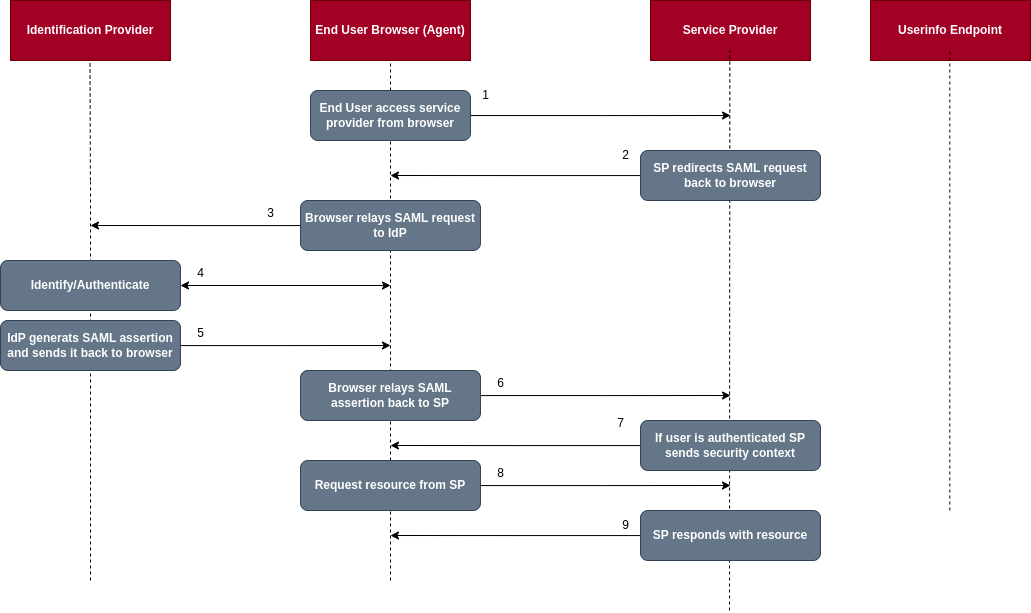
\includegraphics[width=0.4\columnwidth]{saml-flow} 
    \caption{Diagramma di flusso dell'autenticazione con SAML
    https://www.elastic.co/blog/how-to-enable-saml-authentication-in-kibana-and-elasticsearch}
\end{figure}

\subsubsection{OAuth2}
OAuth2 è un protocollo di autorizzazione che consente a un'applicazione di accedere alle risorse di un utente senza richiedere le credenziali dell'utente - e, di conseguenza, senza memorizzarle - nato per assicurare l'accesso sicuro e controllato ai dati di un utente da parte di applicazioni di terze parti.

Funziona attraverso una serie di flussi di autorizzazione, in cui l'utente concede l'autorizzazione all'applicazione per accedere alle sue risorse. L'applicazione, a sua volta, ottiene un token di accesso che può essere utilizzato per accedere alle risorse dell'utente.

Il protocollo OAuth2 è utilizzato da molte grandi piattaforme online come Google, Facebook e Twitter ed è diventato, di fatto, uno standard nei servizi cloud, nei social network, nei servizi di pagamento online e in molti altri contesti.

\begin{figure}[!h] 
    \centering 
    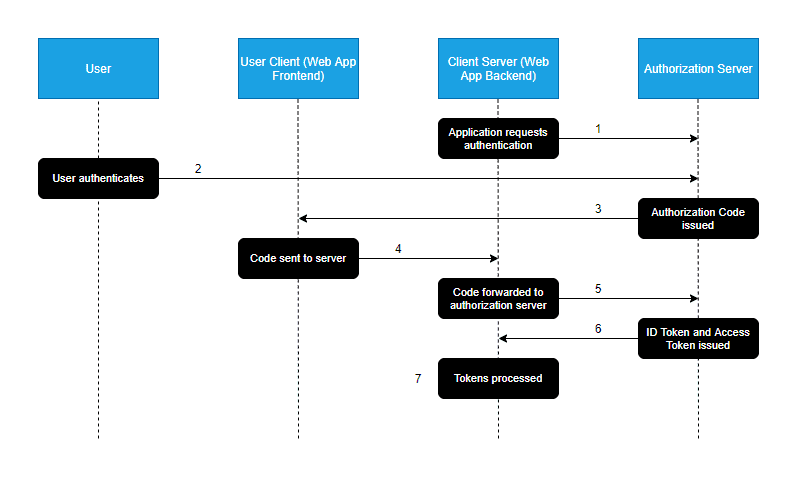
\includegraphics[width=0.4\columnwidth]{oauth2-flow} 
    \caption{Diagramma di flusso dell'autorizzazione con OAuth2
    https://www.loginradius.com/blog/engineering/authorization-code-flow-oauth/}
\end{figure}
\subsubsection{OpenID Connect}
OpenID Connect (OIDC) è un protocollo di autenticazione basato su OAuth2, utilizzato per l'autenticazione degli utenti in applicazioni web e mobile. Progettato per risolvere il problema dell'autenticazione sicura e decentralizzata in applicazioni di terze parti, consente agli utenti di utilizzare l'SSO per accedere a diverse applicazioni, senza, quindi, dover creare un nuovo account per ogni applicazione, bensì delegando l'autenticazione ad un provider esterno (OpenID Provider).

OIDC fornisce un framework standard per l'autenticazione basata su JSON Web Tokens (JWT), in cui l'utente viene autenticato una sola volta e poi viene rilasciato un token di accesso contenente le informazioni di base dell'utente, come l'identificatore univoco, il nome e l'e-mail, che può essere utilizzato per accedere alle risorse protette.

Questo protocollo è stato adottato da molte grandi piattaforme online, tra cui Google, Microsoft e Amazon ed è anche supportato da molte librerie di sviluppo, caratteristica che lo rende semplice da implementare per gli sviluppatori.

\begin{figure}[!h] 
    \centering 
    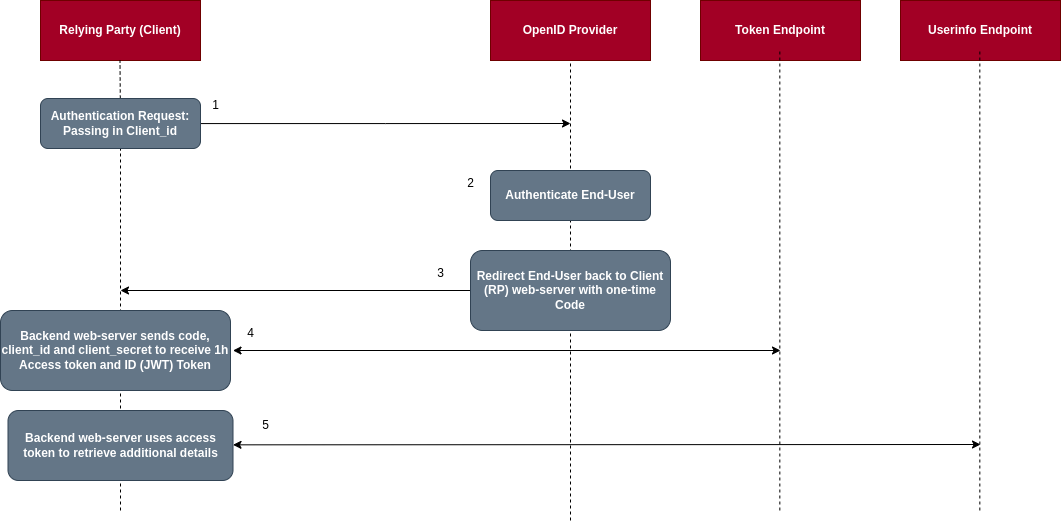
\includegraphics[width=0.4\columnwidth]{oidc-flow} 
    \caption{Diagramma di flusso dell'autenticazione con OIDC
    https://developers.onelogin.com/openid-connect}
\end{figure}

\subsection{Linux PAM}
Linux PAM (Pluggable Authentication Modules) è un framework di autenticazione per i sistemi operativi Linux e UNIX che consente di configurare diversi metodi di autenticazione, come quella tramite password, a due fattori, basata su token, biometrica, ecc.

Utilizzato in una vasta gamma di applicazioni e servizi, tra cui il sistema di login del sistema operativo ed il server SSH, il framework di PAM è composto da una serie di moduli, ognuno dei quali implementa una particolare funzionalità di autenticazione. I moduli PAM sono progettati per essere "pluggable", ovvero possono essere facilmente sostituiti o aggiunti senza dover modificare il codice sorgente del sistema operativo.

L'architettura modulare di PAM consente di creare una catena di moduli, in cui ciascuno dei quali può verificare una parte dell'identità dell'utente. Ad esempio, un modulo può verificare la password dell'utente, mentre un altro può verificare il certificato del client. Se uno qualsiasi dei moduli nella catena fallisce, l'intero processo di autenticazione viene interrotto. Inoltre, è possibile sviluppare dei moduli personalizzati ed integrarli nelle diverse funzioni che richiedono PAM.

\section{Self-Sovereign Identity}

L'SSI (Self-Sovereign Identity) è un nuovo approccio alla gestione delle identità digitali che consente agli utenti di possedere, controllare e condividere le proprie informazioni di identità in modo sicuro e privato. A differenza dei sistemi di identità tradizionali, in cui le informazioni di identità sono conservate in modo centralizzato da terze parti, l'SSI consente agli utenti di essere i proprietari esclusivi dei propri dati di identità digitali.

L'SSI si basa sulla tecnologia blockchain, che consente di creare registri distribuiti di informazioni sicure e immutabili. In tal modo, le informazioni di identità degli utenti vengono conservate in modo decentralizzato e sicuro, senza la necessità di un'autorità centralizzata di controllo.

Per utilizzare l'SSI, gli utenti creano un'identità digitale che include le informazioni di identità necessarie, come nome, indirizzo e informazioni di contatto. Questa identità digitale viene conservata sulla blockchain e protetta da una chiave privata unica, che solo l'utente possiede.

Gli utenti possono utilizzare la propria identità digitale SSI per accedere a servizi online e condividere le proprie informazioni di identità solo con le parti che desiderano. Questo viene fatto attraverso l'utilizzo di un protocollo di scambio di informazioni sicuro e decentralizzato, chiamato DID (Decentralized Identifier).

L'SSI offre numerosi vantaggi, tra cui un maggiore controllo e privacy per gli utenti rispetto ai sistemi di identità tradizionali, una maggiore sicurezza attraverso l'utilizzo della tecnologia blockchain e una maggiore efficienza nella gestione delle identità digitali. Tuttavia, è ancora una tecnologia emergente e richiede una maggiore adozione e sviluppo per diventare un approccio mainstream alla gestione delle identità digitali.
             % 
% !TEX encoding = UTF-8
% !TEX TS-program = pdflatex
% !TEX root = ../tesi.tex

%**************************************************************
\chapter{Configurazione dello stato iniziale}
\label{cap:configurazione-stato-iniziale}
%**************************************************************

\intro{In questo capitolo vengono descritti i procedimenti attuati per configurare lo stato iniziale dei sistemi e utilizzati.}\\

Avendo familiarità con Ubuntu ho, inizialmente, verificato che il pacchetto del server di FreeIPA fosse presente: ho presto appreso che esso era discontinuo sulle ultime versioni del sistema operativo.

Così, ho deciso di optare per \acrshort{centos} Stream 9, ultima versione disponibile, per l'ottima compatibilità con FreeIPA e la migliore usabilità in ambienti server.

A questo punto, con l'aiuto del team di \myAzienda, ho configurato \acrshort{lxc} sulla mia macchina Ubuntu 22.04 \acrfull{lts}.

Tramite il comando \texttt{lxc-create -t download -n ipa-server}, ho creato un nuovo container con il nome di \emph{ipa-server} indicando di voler scaricare il template dalla lista di quelli disponibili, dalla quale ho scelto l'immagine di \acrshort{centos} Stream 9 (\autoref{fig:lxc-template}).

\begin{figure}[!h] 
    \centering 
    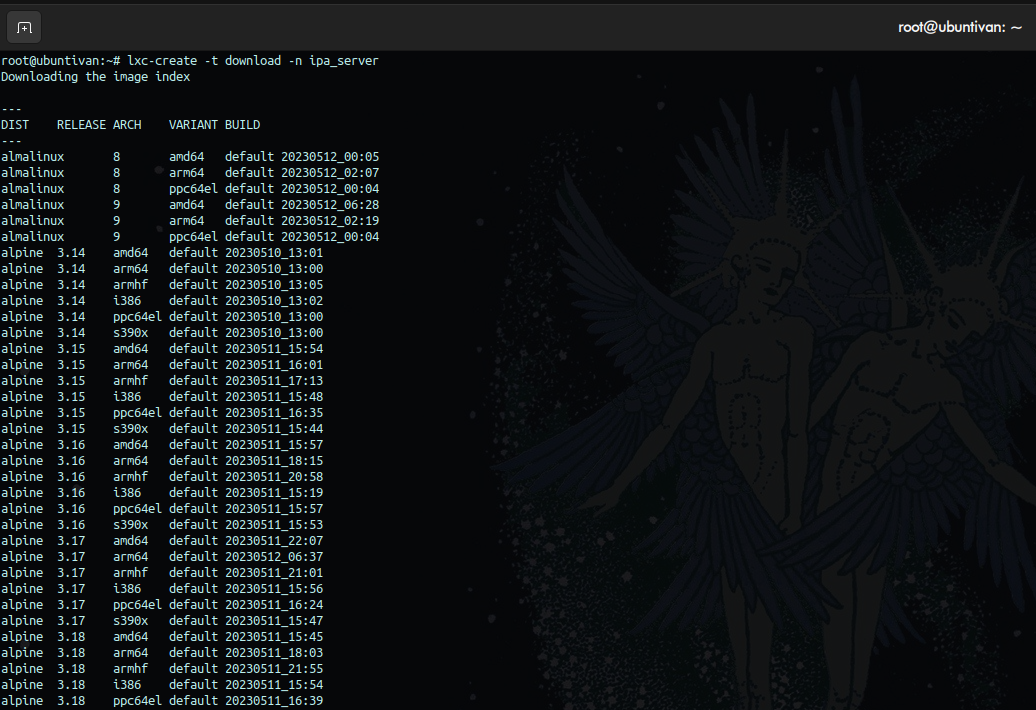
\includegraphics[width=\columnwidth]{lxc-templates} 
    \caption{Vista parziale del template download di \acrshort{lxc}}
    \label{fig:lxc-template}
\end{figure}

Dopo la creazione della macchina ho lanciato i comandi \texttt{lxc-start ipa-server} e \texttt{lxc-console ipa-server}, rispettivamente per avviare il container e per accedere al relativo terminale.


Dopo aver configurato il container per il server ed aver eseguito l'aggiornamento dei pacchetti con il comando \texttt{yum update}, sono passato all'installazione del server di FreeIPA, disponibile su quella release con il pacchetto \emph{freeipa-server}.


Al mio arrivo negli uffici di \myAzienda, l'azienda aveva già configurato per me un account sulla loro piattaforma di testing, \emph{test.monokee.com}, utilizzando come e-mail il mio indirizzo istituzionale e garantendomi l'accesso a tutte le risorse della piattaforma, oltre che alla documentazione aziendale.

Inoltre, avevano predisposto sull'intranet aziendale, tramite Proxmox, delle macchine virtuali \acrshort{centos} e \acrshort{rhel} pronte all'uso.             % 
% !TEX encoding = UTF-8
% !TEX TS-program = pdflatex
% !TEX root = ../tesi.tex

%**************************************************************
\chapter{Ricerca e sperimentazione}
\label{cap:ricerca-sperimentazione}
%**************************************************************

\intro{In questo capitolo viene descritto il processo di ricerca e sperimentazione di una soluzione efficace per l'implementazione dell'\acrshort{sso} nativo}\\

%**************************************************************
\section{Linux Pluggable Authentication Modules}
\label{sec:tecnologie-strumenti}

La prima idea che ho avuto per integrare l'\acrshort{sso} di Monokee via \acrshort{ssh} sul container \acrshort{centos} che ho predisposto è stata quella di creare un nuovo modulo \acrshort{pam}. Ciò perché, studiando i file presenti al percorso \texttt{/etc/pam.d/} ho trovato il file \texttt{sshd}, che stabilisce i moduli da utilizzare per autenticazione, autorizzazione, sessione e gestione della password. In un primo momento mi sono concentrato sulla parte di autenticazione, controllando il file di configurazione \texttt{common-auth}, incluso in \texttt{/etc/pam.d/sshd}, che rappresenta l'autenticazione predefinita di UNIX (con password memorizzata localmente). 

Tuttavia, l'installazione di FreeIPA sovrascrive il parametro \texttt{UsePam yes} del file \texttt{/etc/ssh/sshd\_config} anteponendo dei parametri relativi a Kerberos, in modo da potersi autenticare con la password dell'utente FreeIPA specificato nel prefisso della macchina nel comando di \acrshort{ssh}.

La mia idea era, dunque, quella di rimuovere questi parametri e tornare all'autenticazione via \acrshort{pam}, sostituendo però il modulo predefinito con uno creato appositamente per l'\acrshort{sso} di Monokee.

Il problema restava quello del riconoscimento dell'utente ma avevo già pensato a diversi modi in cui poterlo risolvere, così ho deciso di proseguire e sperimentare con lo sviluppo di un modulo \acrshort{pam} di test, per verificare la fattibilità della mia intuizione.

\subsection{Sviluppo del modulo PAM}
Dapprima, ho deciso di sviluppare una semplice applicazione \acrshort{pam}-aware\cite{site:pam-app}, ovvero compatibile con Linux \acrshort{pam}, utilizzando il linguaggio C e facendo riferimento alla documentazione trovata\cite{site:writing-pam-application}\cite{site:understanding-pam}\cite{site:pam-configuration}\cite{site:linux-man-online}.  

Successivamente, ho sviluppato il modulo \acrshort{pam} di prova\cite{site:pam-module}\cite{site:pam-module-oidc} e l'ho impostato come metodo di autenticazione per l'\acrshort{ssh} con il seguente procedimento\cite{site:writing-pam-module}: prima di tutto, ho modificato il file di configurazione \texttt{/etc/ssh/sshd\_conf} disattivando il parametro \texttt{Set PasswordAuthentication} ed attivando il parametro \texttt{Set Use\acrshort{pam}}; in seguito, ho modificato il file di configurazione dei moduli \acrshort{pam} da utilizzare per il servizio \acrshort{ssh}, \texttt{/etc/pam.d/sshd}, commentando tutte le righe che facevano riferimento all'autenticazione ed inserendo una riga con il nome del modulo di prova che ho sviluppato, etichettato come \texttt{auth  sufficient}, indicando che era sufficiente ottenere esito positivo da tale modulo per autenticarsi con successo. 

\section{FreeIPA Identity Provider}

Dato che la soluzione con il modulo \acrshort{pam} si è rivelata essere più impegnativa del previsto, ho deciso di provare a configurare l'\acrshort{sso} con Monokee da FreeIPA. 

Navigando nell'interfaccia web del software, infatti, ho notato che nella sezione \textit{Authentication} > \textit{Identity Provider Servers} era possibile definire un \acrshort{idp} che utilizzasse \acrshort{oauth2} 2.0 come protocollo di autenticazione\cite{site:freeipa-docs}.

A questo punto, con l'aiuto del team, e, in particolare, del \acrfull{cto} di \myAzienda, mi sono spostato sull'infrastruttura di testing di Monokee per configurare un'applicazione \acrshort{oauth2} da poter utilizzare come Identity Provider per FreeIPA.

             % 
% !TEX encoding = UTF-8
% !TEX TS-program = pdflatex
% !TEX root = ../tesi.tex

%**************************************************************
\chapter{Implementazione e documentazione}
\label{cap:implementazione-documentazione}
%**************************************************************

\intro{In questo capitolo viene illustrato il processo di implementazione della soluzione trovata e la stesura della documentazione relativa.}


\section{Configurazione Monokee}
All'interno dell'ambiente di test di Monokee, tramite l'interfaccia web, ho creato una nuova applicazione \acrshort{oauth2}\footcite{site:oauth-flow} ed un nuovo \acrshort{oidc} provider, che fornisse gli end-point per l'autenticazione via \acrshort{oidc}\footcite{site:monokee-docs}.


\section{Configurazione FreeIPA}
Da FreeIPA, ho proceduto a configurare un nuovo Identity Provider server, tramite la sezione della \acrfull{gui} di cui sopra, inserendo tutte i metadati richiesti, facendo riferimento all'applicazione \acrshort{oauth2} creata su Monokee e agli end-point forniti dall'OpenID provider configurato precedentemente.

Successivamente, ho creato un utente FreeIPA che utilizzasse come unico metodo di autenticazione quella tramite Identity Provider esterno (\emph{External \acrshort{idp}}), scegliendo Monokee come \acrshort{idp} e come identificatore il mio indirizzo e-mail istituzionale, già associato al mio account Monokee, per poter eseguire l'accesso via \acrshort{sso} con le mie credenziali\footcite{site:using-ext-idp-idm}.  

Configurata correttamente l'infrastruttura di autenticazione sia su Monokee che su FreeIPA, ho proceduto a verificarne il funzionamento seguendo le indicazioni della documentazione relativa: dapprima, ho generato un file per l'autenticazione tramite canale FAST con il comando \texttt{kinit -n -c ./fast.ccache}; successivamente, ho richiesto l'autenticazione anonima tramite PKINIT con il comando \texttt{kinit -T ./fast.ccache monokee1}; a questo punto, viene eseguito il flusso di \acrshort{oidc} e viene mostrato un URL al quale autenticarsi tramite \acrshort{sso} di Monokee; ad autenticazione eseguita, basta tornare sul terminale e premere invio per completare l'autenticazione.

Per verificare la corretta autenticazione ho poi lanciato il comando \texttt{klist}, che mostra i ticket Kerberos richiesti, e controllato che l'utente attuale fosse lo stesso con cui volevo autenticarmi e che il ticket fosse valido \autoref{fig:ipa-cli}.  

\begin{figure}[!h] 
    \centering 
    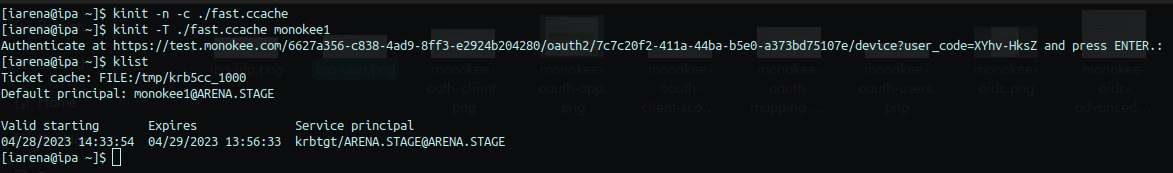
\includegraphics[width=\columnwidth]{ipa-cli} 
    \caption{Autenticazione con Monokee \acrshort{sso} tramite FreeIPA da \acrshort{cli}}
    \label{fig:ipa-cli}
\end{figure}


\section{Problematiche riscontrate}

Durante l'integrazione dell'\acrshort{sso} tramite FreeIPA, nonché già dal processo di configurazione dello stesso, ho riscontrato numerose problematiche.

In primis, a rendere il processo più faticoso del previsto, è stata la mancanza di una  documentazione esaustiva e di informazioni utili in rete in merito alla risoluzione degli errori, dovuta probabilmente alla userbase di FreeIPA, che, benché tale servizio sia lo standard in ambito \acrshort{iam}, è alquanto ridotta.

In secondo luogo, ho riscontrato errori di inconsistenza piuttosto limitanti tra i registri di FreeIPA e quelli di sistema, oltre che difetti di compatibilità della piattaforma con alcune versioni di \acrshort{centos} e \acrshort{rhel}.

Infine, l'autenticazione di FreeIPA tramite Monokee \acrshort{sso} non riesce a sovrascrivere quella di UNIX quando si vuole raggiungere una macchina tramite \acrshort{ssh} su un utente Monokee già configurato sul server. 

\section{Documentazione}

L'azienda ha richiesto la redazione di una guida che illustrare il processo di configurazione del server FreeIPA e dei sistemi di Monokee per l'integrazione del \acrshort{sso} sulle macchine UNIX, per fornire una base documentativa per facilitare le future progressioni e sperimentazioni relative. Ho steso tale documentazione in formato Markdown, versionando il codice sul repository GitHub aziendale fornito da \myAzienda\footcite{site:docs}.
\section{Sviluppi futuri}
A partire dai risultati che ho ottenuto durante l'attività di stage, gli sviluppi futuri possibili sono molteplici.

Innanzitutto, comincerei con il risolvere il problema legati all'accesso alle macchine con il server di FreeIPA installato tramite \acrshort{ssh} su un utente di FreeIPA, e, dunque, per mezzo del \acrshrot{sso} di Monokee. L'\acrshort{sso}, difatti, viene bypassato e viene richiesta la password dell'utente, la quale, di fatto, non esiste perché non è utilizzata da FreeIPA sugli utenti da autenticare con Monokee. 

Dunque, andrei a verificare le impostazioni attive nei file di configurazione di \acrshort{ssh}, come \texttt{/etc/ssh/sshd\_config}.
\\ \\
Risolto questo problema e avendo, quindi, una macchina a cui è possibile accedere tramite \acrshort{ssh} direttamente con un utente Monokee, il prossimo passo potrebbe essere quello di predisporre delle macchine server con le risorse dell'azienda e fornirne l'accesso 
direttamente da Monokee, utilizzando un servizio come Apache Guacamole.

In questo modo, un utente Monokee privilegiato potrebbe accedere a delle macchine server gestire accessi, privilegi ed altro, oppure, nel caso di un utente subordinato, accedere a delle macchine client, gestite da quella server.             % 
% !TEX encoding = UTF-8
% !TEX TS-program = pdflatex
% !TEX root = ../tesi.tex

%**************************************************************
\chapter{Conclusioni}
\label{cap:conclusioni}
%**************************************************************

\intro{In quest'ultimo capitolo vengono riportate le conclusioni e gli esiti dell'attività di stage}\\


%**************************************************************

\section{Raggiungimento degli obiettivi}

L'attività è stata svolta quasi totalmente in linea con la pianificazione prevista: non ci sono stati ritardi di alcun tipo ed il primo periodo, quello di studio delle tecnologie, ha richiesto meno tempo di quanto preventivato, consentendomi, così, di approfondire ulteriormente lo sviluppo delle soluzioni trovate nelle fasi successive.
Ho completato tutti gli obiettivi richiesti con successo, ad inclusione di quelli desiderabili e opzionali: dopo aver implementato con successo l'\acrshort{sso} di Monokee in una macchina \acrshort{centos} utilizzando FreeIPA, ho prodotto la documentazione relativa, illustrando le procedure da seguire per replicare l'integrazione su altre macchine.

%**************************************************************
\section{Conoscenze acquisite}

Grazie allo stage con \myAzienda{} mi sono addentrato in un campo dell'informatica che poco conoscevo, quello della sicurezza. Ho avuto modo di conoscere i concetti e le tecnologie più significative del momento presente in ambito di identità digitale, come la \acrshort{ssi}, il \acrshort{sso} ed alcuni dei protocolli di autenticazione ed autorizzazione più diffusi, apprendendo, anzitutto, cosa significa creare e gestire un'identità digitale e quali sono i rischi di sicurezza legati ad essa. Oltre ad una già ampia formazione teorica, ho avuto anche la possibilità di migliorare le mie competenze in ambito di sistemi UNIX, entrando a contatto con parti di codice che cambiano direttamente il comportamento del sistema operativo, come i moduli \acrshort{pam} e l'\acrshort{ssh}.
Inoltre, ho imparato a creare dei container \acrshort{lxc} dalle immagini messe a disposizione e, successivamente, a configurare un server di Identity and Access Management, quale FreeIPA, modificando anche, in alcuni casi, manualmente dei file di sistema.
Infine, ho messo in atto le conoscenze acquisite nella prima fase dell'attività, in particolare quelle riguardanti il funzionamento di \acrshort{oauth2} ed \acrshort{oidc}, per implementare il \acrfull{poc} richiesto. 

%**************************************************************
\section{Valutazione personale}

Dopo circa trecento ore passate al fianco del team di \myAzienda{} sono convinto di aver acquisito delle conoscenze e delle competenze, non strettamente tecniche, fondamentali per il mio ingresso prossimo nell'industria: questa esperienza, che costituisce la mia prima nell'ambito del percorso che mi appartiene, quello dell'informatica, mi ha permesso di affrontare personalmente e toccare con mano le sfide, i problemi, le metodologie ed i traguardi propri della realtà delle aziende informatiche.

A partire dalla comunicazione, dall'organizzazione e dalla gestione del tempo e delle risorse, arrivando poi agli effettivi processi risolutivi e di sviluppo, sento di aver ricevuto un contributo signifcativo e di essermi messo alla prova, applicandomi al meglio in un ambiente a me quasi del tutto sconosciuto, al di fuori della mia zona di comfort.
Ora, al momento della stesura di questo documento, ripercorrendo ciò che ho fatto durante questa attività di stage, mi rendo conto ancora meglio del valore che essa ha avuto ed ha per me e per la mia carriera.
             % Conclusioni
\appendix                               

%**************************************************************
% Materiale finale
%**************************************************************
\backmatter
\printglossary[type=\acronymtype, title=Acronimi e abbreviazioni, toctitle=Acronimi e abbreviazioni]
\printglossary[type=main, title=Glossario, toctitle=Glossario]
% !TEX encoding = UTF-8
% !TEX TS-program = pdflatex
% !TEX root = ../tesi.tex

%**************************************************************
% Bibliografia
%**************************************************************

\cleardoublepage
\chapter{Bibliografia}

\nocite{*}
% Stampa i riferimenti bibliografici
% \printbibliography[heading=subbibliography,title={Riferimenti bibliografici},type=book]

% Stampa i siti web consultati
\printbibliography[heading=subbibliography,title={Siti web consultati},type=online]


\end{document}
